%% thesis.tex 2014/04/11
%
% Based on sample files of unknown authorship.
%
% The Current Maintainer of this work is Paul Vojta.

\documentclass[masters]{ucbthesis}
\usepackage{biblatex}

% To compile this file, run "latex thesis", then "biber thesis"
% (or "bibtex thesis", if the output from latex asks for that instead),
% and then "latex thesis" (without the quotes in each case).

% Double spacing, if you want it.  Do not use for the final copy.
% \def\dsp{\def\baselinestretch{2.0}\large\normalsize}
% \dsp

% If the Grad. Division insists that the first paragraph of a section
% be indented (like the others), then include this line:
% \usepackage{indentfirst}

% For a masters thesis, replace the above \documentclass line with
% \documentclass[masters]{ucbthesis}
% This affects the title and approval pages, which by default calls this
% document a "dissertation", not a "thesis".

\newtheorem{theorem}{Jibberish}

\bibliography{references}

\hyphenation{mar-gin-al-ia}
\hyphenation{bra-va-do}

\usepackage{graphicx}

\usepackage{chngcntr}
\counterwithout{figure}{chapter}


\usepackage{amsmath} 
\usepackage{amsthm}
\usepackage{amssymb}
\usepackage{amsfonts}
\usepackage{dsfont}
\usepackage{mathtools}

%\newenvironment{example}[1][Example]{\begin{trivlist}
%\item[\hskip \labelsep {\bfseries #1}]}{\end{trivlist}}

%\newtheorem{exmp}{Example}
\usepackage{thmtools}

\declaretheorem[name=Theorem]{thm}
\declaretheorem[style=definition]{example}
\declaretheorem[style=definition]{definition}


%-----------------------------------------------------------------------------
% Special-purpose color definitions (dark enough to print OK in black and white)
\usepackage{color}

% A few colors to replace the defaults for certain link types
\definecolor{orange}{cmyk}{0,0.4,0.8,0.2}
\definecolor{darkorange}{rgb}{.71,0.21,0.01}
\definecolor{darkgreen}{rgb}{.12,.54,.11}

%-----------------------------------------------------------------------------
% The hyperref package gives us a pdf with properly built
% internal navigation ('pdf bookmarks' for the table of contents,
% internal cross-reference links, web links for URLs, etc.)
\usepackage{hyperref}

%\hypersetup{pdftex,  % needed for pdflatex
%  breaklinks=true,  % so long urls are correctly broken across lines
%  colorlinks=true,
%  urlcolor=blue,
%  linkcolor=darkorange,
%  citecolor=darkgreen,
%  }

\hypersetup{pdftex,  % needed for pdflatex
  breaklinks=true,  % so long urls are correctly broken across lines
  colorlinks=true,
  urlcolor=black,
  linkcolor=black,
  citecolor=black,
  }



\usepackage{url}

%% Define a new 'leo' style for the package that will use a smaller font.
\makeatletter
\def\url@leostyle{%
  \@ifundefined{selectfont}{\def\UrlFont{\sf}}{\def\UrlFont{\small\ttfamily}}}
\makeatother
%% Now actually use the newly defined style.
\urlstyle{leo}

% enables straight single quote
\makeatletter
\let \@sverbatim \@verbatim
\def \@verbatim {\@sverbatim \verbatimplus}
{\catcode`'=13 \gdef \verbatimplus{\catcode`'=13 \chardef '=13 }}
\makeatother

% enables backticks in verbatim
\makeatletter
{\catcode`\`=13
\xdef\@verbatim{\unexpanded\expandafter{\@verbatim}\chardef\noexpand`=18 }
}
\makeatother

\newcommand{\CX}{\mathcal{X}}
\newcommand{\PMF}{\mathrm{PMF}}
\newcommand{\PDF}{\mathrm{PDF}}
\newcommand{\CDF}{\mathrm{CDF}}
\newcommand{\N}[2]{\mathcal{N}\left(#1,#2\right)}
\newcommand{\empavg}[2]{\frac{1}{#1}\sum_{i=1}^{#1}\left[#2\right]}
\newcommand{\E}[1]{{\rm I\kern-.3em E}\left[#1\right]}
\newcommand{\Var}[1]{\mathrm{Var}\left[#1\right]}
\newcommand{\Cov}[1]{\mathrm{Cov}\left[#1\right]}
\newcommand{\bias}[1]{\operatorname{Bias}\left[#1\right]}
\newcommand{\sign}[1]{\operatorname{sign}\left(#1\right)}
\newcommand{\df}[1]{\text{df}\left(#1\right)}
\def\ci{\perp\!\!\!\perp}
\newcommand{\argmax}[1]{\underset{#1}{\operatorname{argmax}}}
\newcommand{\argmin}[1]{\underset{#1}{\operatorname{argmin}}}
\newcommand{\iid}{\stackrel{\mathrm{iid}}{\sim}}


\usepackage{algpseudocode}
\algtext*{EndWhile}% Remove "end while" text
\algtext*{EndIf}% Remove "end if" text
\algtext*{EndFor}% Remove "end if" text
\algtext*{EndFunction}% Remove "end if" tex

\newcommand{\reals}{\mathbf{R}}
\newcommand{\ints}{\mathbf{Z}}
\newcommand{\rationals}{\mathbf{Q}}


\usepackage{cancel}

\newcommand\SetSymbol[1][]{\nonscript\:#1\vert\allowbreak\nonscript\:\mathopen{}}
\providecommand\given{} % to make it exist
\DeclarePairedDelimiterX\Set[1]\{\}{\renewcommand\given{\SetSymbol[\delimsize]}#1}

\newcommand{\smallcirc}{\mathbin{\text{\raisebox{0.2ex}{\scalebox{0.6}{$\circ$}}}}}
\newcommand*\dif{\mathop{}\!\mathrm{d}}
\newcommand{\pvalue}{\emph{p}-value}


\begin{document}

\renewcommand\thmcontinues[1]{Continued}
% Declarations for Front Matter

\title{\texttt{permute}---a Python package for permutation tests and confidence sets}
\author{Kenneth Jarrod Millman}
\degreesemester{Spring}
\degreeyear{2015}
\degree{Master of Arts}
\chair{Professor Sandrine Dudoit}
\othermembers{Professor Philip B. Stark \\
  Professor Nicholas P. Jewell}
\numberofmembers{3}
\field{Biostatistics}
% Designated Emphasis -- this is optional, and rare
% \emphasis{Colloidal Telemetry}
% This is optional, and rare
% \jointinstitution{University of Western Maryland}
% This is optional
\campus{Berkeley}

\maketitle
% Delete (or comment out) the \approvalpage line for the final version.
%\approvalpage
\copyrightpage

%% (This file is included by thesis.tex; you do not latex it by itself.)

\begin{abstract}

% The text of the abstract goes here.  If you need to use a \section
% command you will need to use \section*, \subsection*, etc. so that
% you don't get any numbering.  You probably won't be using any of
% these commands in the abstract anyway.

Invasive brag; forbearance.

\end{abstract}


\begin{frontmatter}

%\begin{dedication}
%\null\vfil
%\begin{center}
%To \\\vspace{12pt}
%\end{center}
%\vfil\null
%\end{dedication}

% You can delete the \clearpage lines if you don't want these to start on
% separate pages.

\tableofcontents
\clearpage
%\listoffigures
%\clearpage
%\listoftables

%\begin{acknowledgements}
%\end{acknowledgements}

\end{frontmatter}

\pagestyle{headings}

% (Optional) \part{First Part}

\chapter{\label{ch:intro}Introduction}

\texttt{permute} is a Python package for permutation tests and confidence
sets.\footnote{\url{http://statlab.github.io/permute}}
Philip B. Stark, Kellie Ottoboni, and I developed this package over the
last year with most of the work occurring during the last few months.
In this report, I briefly explain the purpose of the package (\S~\ref{ch:intro}), our
development practices (\S~\ref{ch:dev}), the currently available functionality (\S~\ref{ch:func}), and
our immediate and long-term roadmap (\S~\ref{ch:nextsteps}).

\section{Permutation tests and confidence sets}

Permutation tests (sometimes referred to as randomization, re-randomization, or
exact tests) are a nonparametric approach to statistical significance
testing.  In a permutation test, the distribution of the test statistic under
the null hypothesis is obtained (exactly or approximately) by 
computing the test statistics of all possible relabelings of the observed data.

%For example, imagine you observe 10 coin tosses (e.g., HTTHTHTTTT). Assume 
%each trial is independent and identically distributed and let the
%test statistic be the number of Hs. Under the null hypothesis that the
%coin is unbiased, the Hs and Ts are exchangeable and the expected value of the
%test statistic is 5. To find the distribution of this test statistic under the
%null, count all possible sequences yielding a test statistic of 0,
%1, 2, ..., or 10 Hs in 10 tosses.

For example, consider the following regression problem.  In this case, the
observed data might be 10 $(x, y)$ pairs, which we wish to fit (using least
squares) to a linear model $y = a + bx + \epsilon$.  To test whether $b = 0$,
let's use $\hat{b}/\text{SE}(\hat{b})$ as the test statistic.  Under the null
hypothesis, there is no linear relation between $x$ and $y$, so all possible
combinations of pairs $(x,y)$ are equally likely.  Hence the distribution of
the test statistic is found by computing it on all possible $(x, y)$ formed by
permuting the $y$ values among the $x$ values.

From the distribution of the test statistic under the null, you compute
p-values by taking the ratio of the count of the \emph{as extreme} or
\emph{more extreme} test statistics to the total number of such test
statistics. While there is no analytic expression for this problem, the
computational procedure is straightforward.  Further note that this exact
procedure works regardless of the particular test statistic choosen.

A parameteric approach to this problem would begin by imposing additional
assumptions on the noise $\epsilon$.  For example, if it is assumed that
$\epsilon$ comes from identical Guassian distributions independently realized
for each observed pair, then the test statistic has a $t$-distribution with
$n-2$ degrees of freedom.  If this additional assumption holds, then we can read
the p-value off a table.  Note that, unlike in the permutation test, we were
only able to calculate the p-value (even with the additional assumptions)
because we happened to be able to derive the distribution of this specific
test statistic. 

%For instance, in the first example, the test statistic is 3.
%Under the null, the expected test statistic is 5.  Thus the more extreme test
%statistics are 0, 1, 2, 3, 8, 9, and 10. So the p-value is
%\begin{align*}
%\frac{\binom{10}{0} + \binom{10}{1} + \binom{10}{2} + \binom{10}{3} +
%   \binom{10}{8} + \binom{10}{9} + \binom{10}{10}}{2^{10}}.
%\end{align*}

In summary, the general procedure for computing a p-value using permutation
testing is: 1) carefully formulate the null hypothesis based on the
experimental design and question of interest, 2) from the observed data,
generate all equally likely possible datasets, 3) compute the test statistic
for the observed and generated hypothetical data, and 4) calculate the
proportion of data sets with test statistic at least as extreme as the
observed.  Of course, as the number of observations increases this procedure
may become computationally intractable.  In this case, simulation can often
produce good approximate results.

The advantage of this approach is that it produces exact (or approximately
exact) results using a strong null hypothesis (i.e., we can employee whatever
test statistic we are interested in) and weaker assumptions (since we don't
need to derive an analytic form for the distribution of our choosen test
statistic) about the generating process. Thus permutation testing allows us to
focus on the exact question of interest, rather than a similiar question which
is amenable to analysis.  Additionally, the rationale justifying these claims
doesn't require asymptotic theory; this means it should be easier for
non-mathematically trained scientists to fully understand.  However, the
obvious disadvantage is the computational cost.

What does permute aim to provide
\begin{itemize}
\item experimental design needs to be carefully considered in designing
  permutation tests. We'd like to provide the tools that will enable scientists
  to conduct tests that actually correspond to their experimental design
\item provide Python tools to statisticians, and provide better statistical
  tools to Python users.
\end{itemize}

\section{Python}

Python is a high-level, general purpose programming language, which has become
increasingly popular for scientific computing \cite{millman2011python,
Perez2011}. Unlike some high-level languages used in scientific computing,
Python was not specifically designed for scientific applications.  However, it
quickly attracted interest among scientists and engineers.  Initially, it was
employed primarily as a ``glue'' language to couple together compiled binaries
for scientific applications written in C or Fortran \cite{dubois2007guest}.

As more scientists and engineers began using Python, they started developing
third party libraries to provide additional functionality for scientific
and numeric computing.  In particular, NumPy\footnote{\url{http://numpy.org}},
SciPy\footnote{\url{http://scipy.org}}, and matplotlib\footnote{
\url{http://matplotlib.org}} provide a core foundation on which other
scientific Python packages (such as \texttt{permute}) build. NumPy
provides the basic n-dimensional array data structure and a small core
functionality such as linear algebra routines to compute on this
data structure.  SciPy adds additional general routines on top
of this core functionality necessary for scientific computing including
basic statistics and optimization.  Complementing these data structures
and algorithms, matplotlib provides publication quality 2D plotting.  

While it is beyond the scope of this report to explore these packages in more
detail, I note that the pseudo-random number generator (PRNG) provided by NumPy
is the Mersenne Twister.  The Mersenne Twister is an efficient PRNG with a
sufficiently large period for most statistical simulations.\footnote{It is
default PRNG in R as well.  While sufficient for most statistical simulations,
for other applications such as cryptography it may be insufficient.}  In
addition to providing a high-quality PRNG, NumPy implements Knuth shuffling ---
an efficient (and simple) algorithm for uniformly generating permutations of
sequences.

While Python is similar to R in many respects and is widely used in scientific
and numerical computing, it lacks R's extensive support for statistical
applications.  Recently, however, it has become more attractive for statistical
applications due to new packages such as Pandas, statsmodels, and
scikit-learn.  Our intention is to help accelerate this trend by supplying a
high-quality, rigorously tested, and statistically sound package for a large
variety of permutation tests and confidence sets. As the package matures, we
anticipate contributing generic functionality upstream to the packages we
depend on as appropriate.

\chapter{\label{ch:dev}Development practices}

As this is a new software project, we invested a significant effort in setting
up a development infrastructure to ensure our work is carefully tracked,
thoroughly and continually tested, and incrementally improved and documented.
To this end, we have adopted best practices for software development used by
successful open source projects \cite{millman2014}.

\section{\label{sec:vc}Version control}

We use Git\footnote{\url{http://git-scm.com}} as our version control
system (VCS) and GitHub\footnote{\url{https://github.com}} as the public hosting
service for our official \texttt{upstream} repository.  Git allows us to
carefully track how our code evolves as well as deliberately consider and
refine new functionality on isolated branches before merging it into the main
branch.

\subsection{Git data model}

Git's data model is sufficiently different from other VCS that it is helpful to
briefly describe it before discussing our Git workflow.  In Git, a repository
is represented as a directed acyclic graph (DAG) of commits.  A commit in Git
is a cryptographically signed object containing zero or more parent commits,
some metadata, and a snapshot of entire work tree.  A working tree can be
thought of as the entire project structure of directories and files at a
particular point in the development.  Over time the working tree evolves due to
new features, refactoring of current functionality, optimizations, or bug
fixes.  Taking snapshots of this evolution over time allows us to analyze the
past to better understand how the code came to be in its present state.  The
cryptographic signature ensures that it is practically impossible for someone
to change history without it being readily apparent.\footnote{Surprisingly
few previous VCS even attempted to ensure the historical integrity of a
project's history.}

An essential design feature of Git (and one absent from other VCS), is
the simplicity of creating and merging branches.  A branch in Git is a pointer
to a commit in the repository DAG, which moves forward as new commits are made.
This provides a lightweight mechanism for branching.  Typically each repository
has a master branch which is viewed as the main truck of development.  Creating
a new branch off the master branch (or main trunk) only requires making a new
label and then committing to it.  A merge is a commit with 2 or more parents,
which corresponds to the resulting integration of the parent commits.

Further, Git is completely decentralized so there are no inherent
asymmetries as found in older client-server models.  So every developer
has their our own self-contained repository.  For collaborative purposes,
Git repositories have a notion of remote repositories.  Remotes are other
repositories that a specific repository tracks.  Commits can be pushed
and pulled from remote repositories into local repositories.

Git, while not easy to master, is simple in the sense that once a few concepts
are understood, it behaves in an entirely reliable, intelligible, and
straightforward manner.\footnote{To clarify the distinction I am making between
easy and simple, let me use the familiar example of Calculus.  Many students
require one or more semesters of college level coursework to learn the basic
techniques of differentiation and integration.  In this sense, it isn't easy to
learn.  However, once the basic techniques are learned, it is simple to apply
to new contexts and applications.  Prior to the invention of Calculus,
discovering how to compute the area under a new curve often required
mathematical genius and insight into the specific application.} If you've ever
tried to do anything non-trivial in ``easier'' to use VCS such as SVN or CVS,
then you've likely experienced the ensuing frustration these systems cause.
More likely you've never tried to do anything non-trivial with such systems as
it is completely unclear how such things could be done.  With Git the pain is
upfront, but the benefits are extensive and enable fluid and comprehensive
collaborations, which scale well.

The inherent flexibility of Git makes numerous workflows possible.  We've
followed the standard workflow used by the core scientific Python packages.
This workflow enables us to keep the official master branch of the project in a
pristine state at all times and simplifies the structure of the DAG by
divorcing it from the sometimes random, tentative moves made when developing
new code so that we can record a revised and coherent history.  Further it
rationalizes the process of making changes to the official master by allowing
us to add new features and bug fixes in isolated, tested, and code reviewed
chunks.

We've designated \url{https://github.com/statlab/permute} as the official
upstream master.  No one commits changes to it directly.  Instead we each fork
this repository on GitHub (e.g, my fork is
\url{https://github.com/jarrodmillman/permute}).  To fork a project on GitHub,
you click a button labeled fork on the repository website you wish to fork.
This let's GitHub track the relationship between various repositories it hosts.
In particular, it enables you to create pull requests, which I discuss below.

Once we've forked the official repository, we clone our fork onto a local
account so we can work on the code.  Rather than work on the \texttt{master}
branch of our repositories, we perform all code changes on branches.  As
we work on our branch we push the changes to our individual forks.  Once
we've pushed our branch to our fork on GitHub, we can create a pull request
to begin the code review process necessary to merge our branch into the
upstream master.

To get new code integrated in the official \texttt{upstream} master, we use
GitHub's \emph{pull request} mechanism.  This helps make performing code review
for new code added to the official ``upstream'' repository easy to manage.
Given the short development history and small development team, we have
kept the review process lightweight and mostly automated, which I describe
below.

Once a \emph{pull request} is reviewed and accepted, it is merged into
the upstream master.  Once merged into the upstream repository, we pull
the changes into our local repository and then cleanup after ourselves.

To summarize, all new work is made on a branch and pushed to our
personal forks of the upstream repository. To incorporate this new
work on our local master branch we then pull from the upstream
master.  This separation between where we push and pull our
work creates the space for code review, testing, and discussion of
new features and bugfixes before merging work into the official 
repository.

\section{\label{sec:test}Testing}

We use the \texttt{nose} testing framework for automating our testing
procedures.\footnote{\url{https://nose.readthedocs.org}}  This is the standard
testing framework used by the core packages in the scientific Python ecosystem.
Automating the tests allows us to monitor a proxy for code correctness when
making changes as well as simplifying the code review process for new code. 

The \texttt{nose} testing framework simplifies test creation, discovery,
and running. It has an extensive set of plugins to add functionality
for coverage reporting, test annotation, profiling, isolation, as well
as inspecting and testing documentation.

So far, we've primarily used it for testing individual units of code for
consistency.  Eventually we will add regression and integration testing as well
as testing the code for correctness using the expected statistical properties.
For instance, rather than merely checking whether when a function is called
with the same arguments it returns the same results, we can run tests that
check whether results are within the expected statistical error.

%While testing is not a proof of program correctness, it can serve as a
%useful tool for catching errors and increase our confidence in the
%reliability of our results.

%For example, from the top-level of the repository, you can ask \texttt{nose}
%to run the tests by entering \texttt{nosetests permute} in Bash.  For example,
%
%\begin{verbatim}
%$ nosetests permute
%.......................................
%----------------------------------------------------------------------
%Ran 39 tests in 48.957s
%\end{verbatim}
%
%In the above console output, you will see a ``.'' for each test, which
%is run.  A test corresponds to a function and each test may test several
%things.

%\subsection{Coverage}

We also use \texttt{nose} to monitor our test coverage.  Our goal is to
test every line of code.  For example, not only do we want to test every
function in our package, but if a specific function has internal logic
we want to test each possible path through the function.  Having tested
each line of code increases our confidence in our codebase, but more
importantly provides us assurance that changes we make do not break
existing code.  It also increases our confidence that new code works,
which reduces the friction of accepting contributions.

%Working in the top-level of our local repository in Bash, you could
%enter
%
%\begin{verbatim}
%$ nosetests permute --with-coverage --cover-package=permute
%.......................................
%Name                 Stmts   Miss Branch BrMiss  Cover   Missing
%----------------------------------------------------------------
%permute                 43      5     10      1    89%   77-88
%permute.core            60      0     30      4    96%   
%permute.data            45      0      2      0   100%   
%permute.eda             22      0      8      0   100%   
%permute.irr             52      0     20      1    99%   
%permute.stratified      45      0     16      1    98%   
%permute.utils           10      0      6      0   100%   
%----------------------------------------------------------------
%TOTAL                  277      5     92      7    97%   
%----------------------------------------------------------------------
%Ran 39 tests in 56.023s
%
%OK
%\end{verbatim}
%Here you can see, that in addition to running 39 tests without error,

Currently over 97\% of our code has at least one test touch it.  The remaining
lines are mostly branch misses where executing both branches is difficult.  For
example, the branch depends on the particular environment in which it is being
run. So each branch is tested in different environments, but not at the same
time.  I've tried to trick the tests to run both branches by hand modifying
system objects in the tests as well as creating mock objects, but haven't been
able to achieve 100\% coverage.

%\subsection{Continuous integration}

Having an automated test suite enables us to implement continuous integration.
Continuous integration is the process of automatically running the full test
suite using different versions of our dependencies (e.g., Python 2 and 3) on
different operating systems (e.g., Windows, Mac OS, and Linux) and different
hardware (e.g., Big-endian and Little-endian systems) every time any new commit
is made to a repository or pull request.

We've configured Travis CI\footnote{\url{https://travis-ci.org}} and
\texttt{coveralls}\footnote{\url{https://coveralls.io}} to be automatically
triggered whenever a commit is made to a pull request or the upstream
master directly.  These systems run the full test suite and generate reports.
These systems are integrated with GitHub so that our pull requests are
automatically annotated with these reports as soon as changes are made.

%Python 2 and Python 3 on Debian-derived system
%
%I run the tests for both Python 2 and Python 3 on a RedHat-derived system
%
%While Philip and Kellie run the tests for Python 2 on Mac OS.
%
%need to add additional build systems to buildbot nipy.bic.berkeley.edu...
%
%\texttt{coveralls}\footnote{\url{https://coveralls.io}}
%
%\begin{figure}
%  \begin{centering}
%    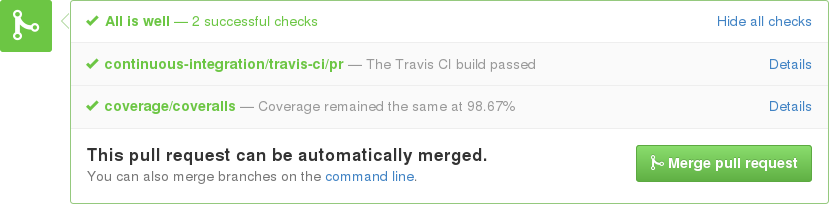
\includegraphics[width=5.5in]{fig/pull-request-ci.png}\par
%  \end{centering}
%
%  \caption{\label{fig:pull-request}Pull request and continuous integration.}
%\end{figure}

\section{\label{sec:doc}Documentation}

Reducing the
friction involved with producing documentation encourages developers and users
to contribute documentation.  For instance, NumPy use to have fairly poor
documentation until one summer when Stefan van der Walt (now a BIDS fellow)
built on several newly improved Python technologies for documentation
\cite{SciPyProceedings_27}.

We've adopted this system and already have good developer documentation and the
foundation for high-quality user documentation. We've used Python docstrings and
the NumPy docstring standard to document all the modules and functions in
\texttt{permute}.\footnote{https://github.com/numpy/numpy/blob/master/doc/HOWTO\_DOCUMENT.rst.txt}

Using Sphinx and some NumPy extensions, we have a system for autogenerating the
project documentation (as HTML or PDF) using the docstrings as well as
stand-alone text written in a light-weight markdown-like language.  This
enables us to embedded references, figures, code that is auto-run during
documentation generation, as well as mathematics using \LaTeX.

\section{\label{sec:release}Release management}

Our development workflow ensures that the official upstream master is always
pristine and ready for use.  This means anyone can get our official upstream
master at any point, install it and start using it.  However, it is still
desirable to periodically make official releases with binary packages uploaded
to PyPI (the Python version of CRAN) and release announcements posted to
community lists.

Since the project is still new, there's only been one release so far.  To install
this release without downloading the source code, you can enter the following
command from a Bash prompt:
\begin{verbatim}
pip install permute
\end{verbatim}
This will install version 0.1.alpha0 of \texttt{permute} as well as it
dependencies.  Since we have yet to finalize our call signatures or package
structure, we use the alpha designation to telegraph this fact to
potential users.  However, our release process is fully documented and
partially automated.  Together with the policy of keeping upstream master
pristine, this means that making new releases is extremely light-weight.  Being
able to quickly generate new releases quickly and reliably is essential to being able to
quickly respond to mistakenly broken releases.  Despite using a rigorous
testing and integration methodology, error is a constant concern.  Being able
to quickly respond to discovered errors in released software is essential to
creating a software tool people trust.

\chapter{\label{ch:func}Current functionality}

While the scope of our package is large, we have initially focused on a
few features.  In particular, we have implemented built-in data sets,
functions for exploratory data analysis, core functionality like various
types of permutations and confidence intervals, some stratified tests
and confidence sets, and a test for interrater reliability.

\section{Data}

To simplify testing as well as providing some standard datasets for
users to experiment with as they learn how our software works, we
have a data module, which provides quick and ready access to a few
builtin data sets. At this point, the majority of the datasets come
from the examples used in ``Permutation tests for complex data: theory,
applications and software'' \cite{pesarin2010permutation}.  These
datasets are discussed in more details in \S~\ref{sec:book}.  We also
have a data set, which we use as an example for the interrater
reliability test (\S~\ref{sec:irr}).

Loading one of the packaged data sets involves importing and then
invoking a helper function, which handles the data loading.  For
example, here is how you would load the data set used for the
interrater reliability test:
\begin{verbatim}
In [1]: from permute.data import nsgk

In [2]: x = nsgk()
\end{verbatim} 

\section{Exploratory data analysis}

As we've added data sets, we've also incrementally added tools to simplify
exploratory data analysis (EDA).  Currently, we provide two helper functions.
One for reporting duplicate rows in a matrix in various formats.  Another for
reporting duplicate consecutive rows in a matrix in various formats.  Rather
than having a list of planned EDA functionality, we have been opportunistic
and have only implemented functionality as needed for data sets we are adding
to the \texttt{data} module.

\section{Core tools}

The \texttt{core} module contains basic functions that could be useful in
multiple specific permutation tests.  

This module provides functions for permuting various data structures in
different ways.  Currently we have functions for permuting the rows of
a matrix in-place as well as permuting conditions within each group.


Compute the confidence interval for a binomial.


Simulate permutation p-value for Spearman correlation coefficient


One-sided or two-sided, two-sample permutation test for equality of two means,
with p-value estimated by simulated random sampling with reps replications.

Tests the hypothesis that x and y are a random partition of x,y against the
alternative that x comes from a population with mean

a. greater than that of the population from which y comes, if side = ‘greater’

b. less than that of the population from which y comes, if side = ‘less’

c. different from that of the population from which y comes, if side = ‘two-sided’

\section{Stratified permutation testing}

\subsection{Problem}

\subsection{Method}

\section{\label{sec:irr}Interrater reliability}

\subsection{Problem}

\cite{davies1982measuring, mchugh2012interrater}

\subsection{Method}

The test statistic within stratum $s$ is

\begin{align*}
\rho_s &\equiv \frac{1}{N_s {R \choose 2}} \sum_{i=1}^{N_s}
              \sum_{r=1}^{R-1} \sum_{v=r+1}^R 1(L_{s,i,r} = L_{s,i,v}) \\
       &= \frac{1}{N_s R(R-1)} \sum_{i=1}^{N_s}
                (y_{si}(y_{si}-1) + (R-y_{si})(R-y_{si}-1)).
\end{align*}

That is, within each stratum, we count the number of concordant pairs of
assignments.


\chapter{Conclusion}

\section{Next steps}


\printbibliography

\appendix
\chapter{\label{app:def}Groups, actions, and orbits}
\setcounter{example}{0}

Groups are a basic object of study in abstract algebra and
are useful in many areas outside of mathematics \cite{armstrong1997groups, dummit2003abstract, lang2002algebra}.  They are intimately
related to the notion of symmetry.

\begin{definition}
A \emph{group} $(G, \cdot)$ is a set $G$ and a binary operation $\cdot: G \times G \to G$
called (group) \emph{multiplication} such that
\begin{enumerate}
\item $ab \in G$ for all $a, b \in G$ (i.e., $G$ is \emph{closed} under multiplication),
\item for all $a, b, c \in G$, $(ab)c = a(bc)$ (i.e., multiplication is \emph{associative}),
\item there exists an \emph{identity} element $e \in G$ such that $eg = ge = g$ for all $g \in G$, and
\item for each $g \in G$ there exists an \emph{inverse} element $g^{-1} \in G$ such that $g^{-1}g = gg^{-1} = e$.
\end{enumerate}
\end{definition}

Given a group $(G, \cdot)$, a subset $H$ of $G$ is called a subgroup if $(H, \cdot)$ is a group
under the multiplication of $G$.  The integers under
addition $(\ints, +)$ is a group with identity element $0$ and where the
inverse of $z$ is $-z$.  The even integers are a subgroup of $(\ints, +)$.
The rational numbers excluding $0$ under multiplication
$(\rationals\setminus \Set{0}, \cdot)$ is a group with identity element $1$ and
where the inverse of $p/q$ is $q/p$. In both cases, it is easy to verify that
the group properties are met.  Here is a more complicated example that we will
use in the sequel. 

\begin{example}
A permutation of an arbitrary set $\CX$ is a bijection from $\CX$ to itself.  The
set $S_\CX$ of all permutations of $\CX$ under function composition
$(S_\CX, \smallcirc)$ is a group.  The associativity of permutations follows from the
associativity of function composition.  The bijection taking every element of
$\CX$ to itself is the identity permutation. Since a permutation is a bijective function, the
inverse of every permutation exists and operates from both left and right.  
If $\CX = \Set{1, 2, \dots, n}$, then $S_\CX$ is the symmetry group of order $n$
and is usually denoted $S_n$.
\end{example}


\begin{definition}
Let $G$ and $H$ be groups.  A \emph{homeomorphism} $\varphi: G \to H$ takes multiplication
from $G$ to $H$ such that $\varphi(xy) = \varphi(x)\varphi(y)$ for all $x, y \in G$.
\end{definition}

Note that the multiplication on $G$ and the multiplication on $H$ may be different operations
and in general $\varphi(x)y$ will be undefined.
To make that explicit, let $(G, \star)$ and $(H, \diamond)$ be groups then we write the
condition for a function $\varphi: G \to H$ to be a homeomorphism as
$\varphi(x \star y) = \varphi(x)  \diamond \varphi(y)$.  
Since the context will make clear the group multiplication being used, we will not usually
distinguish the different  operators.
A homeomorphism takes the identity of $G$ to the identity of $H$
since $\varphi(g) = \varphi(ge) = \varphi(g)\varphi(e)$ for all $g \in G$. It takes inverses to 
inverses since $\varphi(e) = \varphi(g^{-1}g) = \varphi(g^{-1})\varphi(g)$ for all $g \in G$.
If $\varphi$ is a bijection, then it is called an isomorphism.

\begin{definition}
An \emph{action} of a group $G$ on a set $\CX$ is a homeomorphism $\varphi: G \to S_\CX$.
\end{definition}

We say \emph{an} action since a group $G$ can act on $\CX$ in more than one way. Recalling the
definition of a homeomorphism, this means that $\varphi(xy) = \varphi(x)\varphi(y)$ for all
$x, y \in G$ where $\varphi(xy), \varphi(x), \varphi(y) \in S_\CX$.  Also notice that
$\varphi(x)\varphi(y)$ represents composition of the permutations $\varphi(x)$ and 
$\varphi(y)$.  Moreover, $\varphi(e)$ is the identity permutation in $S_\CX$.
It is standard to write $gx$ instead of $\varphi(g)(x)$ since it is more compact.
Note that $gx$ is not ``multiplying'' an element $g$ of $G$ with an element $x$ of $\CX$,
but represents the group action
of $g$ on $x$, which can be thought of as the image of $x$ under the permutation of $\CX$
induced by $g$.  Each $g \in G$ corresponds to a permutation of $\CX$ defined by the
homeomorphism.

%\begin{definition}
%An \emph{action} of a group $G$ on a set $\CX$ is a set of permutations $\pi_g: \CX \to \CX$ for $g \in G$ such that
%
%(1) $\pi_e$ is the identity (i.e., for every $x \in \CX, \pi_e(x) = x$) and
%
%(2) for every $g_1$ and $g_2$ in $G$, $\pi_{g_1} \smallcirc \pi_{g_2} = \pi_{g_1g_2}$.
%\end{definition}



\begin{definition}
The \emph{orbit} $G(x) \equiv \Set{gx  \given g \in G}$ of any $x$ in $\CX$ is
the set of all images of the particular point $x$ under all elements of $G$.
\end{definition}

%The set of all the points in an orbit form an equivalence relations under the group action.
%The set of all such equivalence relations partitions $\CX$ by a subgroup of
%$S_\CX$ under composition endowed with the group structure of $G$.

\begin{example}
The additive group $(\ints, +)$ acts on the real line $\reals$ by translation.
That is, for every integer $z$ and any real number $x$ the group action is given
by $x \mapsto z + x$. To show that this a homeomorphism $\varphi : (\ints, +) \to (S_\reals, \smallcirc)$,
note that given any two integers $m$ and $n$ and any real number $x$ the following
holds $(m + n) + x = m + (n + x)$.  The orbit of $\pi$ (i.e., $3.14152...$) under
this group action is
\begin{align*}
\Set{z\pi  \given z \in \ints} = \Set{z + \pi  \given z \in \ints} =\Set{\dots, 2.14152..., 3.14152..., 4.14152..., \dots}.
\end{align*}
In a similar fashion, the orbit of any real number $x$ under this action of $(\ints, +)$
on $\reals$ creates and equivalence relation under the group structure of $(\ints, +)$ such
that $x \sim y$ with $y$ in $\reals$ exactly when there exists a $z$ in $\ints$ such that
$y = z + x$.
\end{example}

The set of all orbits as $x$ ranges over $\CX$ is a partition of $\CX$ into equivalence classes.
The relevance for permutation tests is as follows: Suppose that $\CX$ is the outcome
space of some experiment, and we will make an observation $X$ drawn from $P$.
Let $(G, \cdot)$ be a group that acts on $\CX$.
Suppose that under the null hypothesis, all elements of $\CX$ in any given orbit under $G$ 
are equally likely.
Then if we observe $X=x$, it is just as likely that we would have observed $gx$ for any
$g \in G$: conditional on the orbit $Gx$, all elements of $Gx$ are equally likely.
This then determines the (conditional) distribution of $X$: every element of $Gx$ is equally
likely given $GX = Gx$---even though we do not know $P(X \in Gx)$.
The uniform conditional distribution lets us calculate the conditional null distribution of
any test statistic.

\begin{thm}
Given a probability space $(\mathcal{X}, \Sigma, \mu)$ and a group $(G, \cdot)$
acting on $\mathcal{X}$ such that $\Sigma$ is closed under the action of $G$,  
let $X \sim P$ for some unknown $P$ dominated by $\mu$.
Consider testing the hypothesis that $P$ is invariant under $G$
\begin{align*}
H_0: P(S \subset \mathcal{X}) = P(GS  \subset \mathcal{X}) \text{  for all }S \in \Sigma.
\end{align*}
Suppose we have a family of tests with (conditional) level no greater than $\alpha$ conditional on the orbit of
the observed data
\begin{align*}
P(\text{reject }H_0 \mid GX=Gx \parallel H_0) \le \alpha,
\end{align*}
where the notation ``$\, \parallel H_0$'' means ``assuming $H_0$ is true.''
Then the resulting overall test has unconditional level no greater than $\alpha$
\begin{align*}
P(\text{reject }H_0  \parallel H_0) \le \alpha.
\end{align*}
\end{thm}

\begin{proof}
By the law of total probability, we have
\begin{align*}
P(\text{reject }H_0  \parallel H_0) &= \int_\mathcal{X} P(\text{reject }H_0  \mid GX=Gx \parallel H_0)P(GX=Gx \parallel H_0) \dif \mu(x) \\
  &\le \int_\mathcal{X} \alpha P(GX=Gx \parallel H_0) \dif \mu(x) \\
  &= \alpha \int_\mathcal{X} P(GX=Gx \parallel H_0) \dif \mu(x) \\
  &= \alpha.  \qedhere
\end{align*}
\end{proof}

\chapter{\label{app:ex}Software demonstration}

For the following two worked examples, we assume that the following imports 
have been made.

\begin{verbatim}
>>> import numpy as np
>>> from scipy import stats
>>> import matplotlib.pyplot as plt
\end{verbatim}

You will also need to have \texttt{permute} version \texttt{0.1a1} installed.

\begin{verbatim}
>>> import permute
>>> permute.__version__
'0.1a1'
\end{verbatim}

Note that this is an \emph{alpha} release, so we are making no claims
regarding the stability of our package structure or call signatures.  We do not
have plans to break our API, but we are allowing ourselves to continue refining
our API as we gain experience using the package and continue adding new
functionality.  However, the following example sessions will give you an idea
of what working with \texttt{permute} is like.

\section*{Two sample permutation test}

There is growing evidence of gender bias in student evaluations of teaching.
To address the question ``Do students give higher ratings to male teachers?,''
an online experiment was done with two professors, one male and one female
\cite{macnell2014s}.  Each professor taught two sections. In one section, they
used a male name.  In the other, they used a female name. The students didn't
know the teacher's real gender.  We test whether student evaluations of
teaching are biased by comparing the ratings when the professor used a male
name versus a female name.

First let us consider the parametric two-sample t-test.  In this case, our
test statistic is
\begin{align*}
t &= \frac{\text{mean(rating for M-identified prof) - mean(rating for F-identified prof)}}{\sqrt{\text{pooled SD of ratings}}}
\end{align*}
For the two-sample t-test, the null hypothesis is that the reported/perceived
teacher gender has no effect on teacher ratings.  The alternative hypothesis
is that teacher ratings differ by reported/perceived teacher gender.  For the
two-sample t-test to be valid, we require the following assumptions:
\begin{itemize}
\item Ratings are normally distributed.  (But they are on a Likert 1-5 scale,
      which is definitely not normal.)
\item Noise is zero-mean and constant variance across raters.  (How should we interpret
      ``noise'' in this context?  Besides constant variance is not plausible: some
      raters might give a range of scores, other raters might always give 5.)
\item Independence between observations. (Students might talk about ratings with
      their peers in the class, creating dependence.)
\end{itemize}

Despite the problematic assumptions we are required to make, let's temporarily
assume they hold and calculate a ``$p$-value'' anyway.

\begin{verbatim}
>>> from permute.data import macnell2014
>>> ratings = macnell2014()
>>> maleid = ratings.overall[ratings.taidgender==1]
>>> femaleid = ratings.overall[ratings.taidgender==0]
>>> df = len(maleid) + len(femaleid) - 2
>>> t, p = stats.ttest_ind(maleid, femaleid)
>>> print 'Test statistic:', np.round(t, 5)
Test statistic: 1.54059
>>> print 'P-value (two-sided):', np.round(p, 5)
P-value (two-sided): 0.1311
\end{verbatim}
Note that the computed ``$p$-value'' is above the standard cut-offs for
reporting significance in the literature.

For the permutation test we can use the same test statistic, but we will
compute the $p$-value by randomly sampling the exact distribution of the test
statistics.  The null hypothesis is that reported/perceived teacher gender has
no effect whatsoever on ratings---as if ``male'' and ``female'' are randomly
assigned labels.  The alternative hypothesis is that reported/perceived teacher
gender has some effect on ratings.  The only assumption we need to make is that
randomization is fair and independent across units.  This can be verified
directly from the experimental design.

\begin{verbatim}
>>> from permute.core import two_sample
>>> p, t, ci, dist = two_sample(maleid, femaleid, stat='t',
...                             interval='two-sided', keep_dist=True)
>>> print 'Test statistic:', np.round(t, 5)
Test statistic: 1.82159
>>> print 'P-value (two-sided):', np.round(p, 5)
P-value (two-sided): 0.04436
>>> print '95% Confidence Interval for the P-value', np.round(ci, 5)
95% Confidence Interval for the P-value [ 0.04309  0.04565]
\end{verbatim}

Not only is the use of this $p$-value justified (since our assumptions are
met), but its value is below the cut-off for significance commonly used.
Since the permutation test also returns the approximately exact distribution
of the test statistic, let's compare the actual distribution with the
$t$-distribution.

\begin{verbatim}
>>> n, bins, patches = plt.hist(dist, 20, histtype='bar')
>>> plt.axvline(x = t, color = 'red')
>>> x = np.linspace(stats.t.ppf(0.0001, df),
                    stats.t.ppf(0.9999, df), 100)
>>> plt.plot(x, stats.t.pdf(x, df)*(100000/2.0), lw=2, alpha=0.6, label='t pdf')
>>> plt.show()
\end{verbatim}

In Figure~\ref{fig:figure1}, you can see the simulated distribution of the test
statistic under the null with the $t$-distribution superimposed on it.

\begin{figure}
  \begin{centering}
    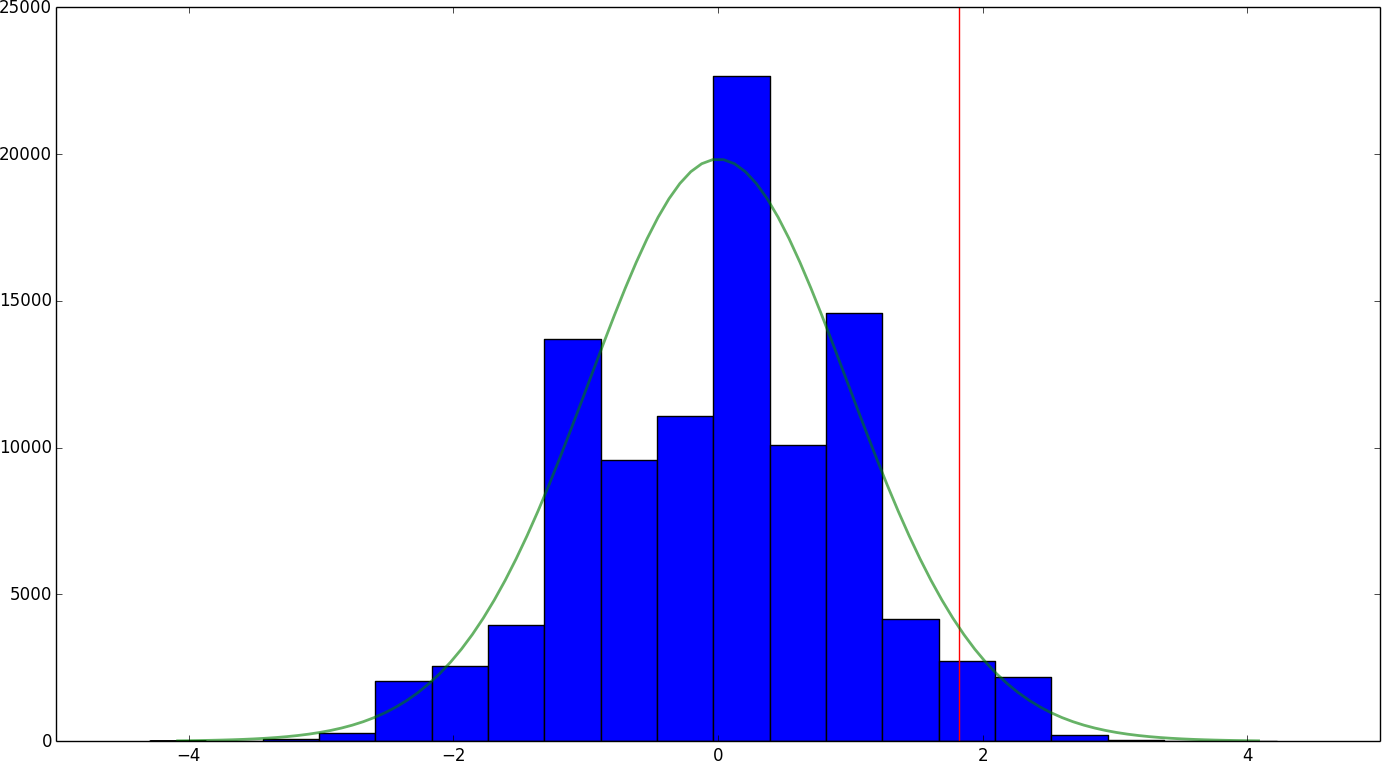
\includegraphics[width=.8\textwidth]{fig/figure_1.png}\par
  \end{centering}

  \caption{\label{fig:figure1}Permutation Null Distribution.}

\end{figure}

\section*{Stratified Spearman correlation permutation test}

To illustrate the use of one of our stratified tests, I will use fake
data similar to that used in \cite{boring2015}; we are unable to use
the actual data due to data privacy laws in France.

The scientific question of interest is now ``Do students' evaluations of
teachers measure teaching effectiveness?''  To answer this question, we were
able use final exam performance as a proxy for value added by
teacher---students have different teachers but take the same final exam.
Our null hypothesis is that there is no association between a student's final
exam performance and the rating they give their professor.  The alternative
hypothesis is that there is a positive association between a student's final
exam performance and the rating they give their professor.

There are 8 professors, each with multiple student ratings.  One might think
that a certain professor gets consistently high reviews because of something (e.g.,
gender, attractiveness, likeability) unrelated to teaching effectiveness.
Stratifying by professor allows us to assess teaching effectiveness for each
individual student.  The test statistic we use within groups is the Spearman
correlation.

\begin{verbatim}
>>> from permute.stratified import sim_corr
>>> evals = np.recfromcsv("SET2.csv")
>>> rho, plower, pupper, pboth, sim = sim_corr(x=evals.rating, y=evals.final,
...                                            group=evals.prof_id)
>>> print 'Test statistic:', np.round(rho, 5)
Test statistic: 0.94787
>>> print 'One-sided (upper) P-value:', np.round(pupper, 5)
One-sided (upper) P-value: 0.18
\end{verbatim}

Finally, I plot the simulated distribution of the test statistics under the null
conditioned on the observed data in Figure~\ref{fig:figure2}.

\begin{verbatim}
>>> n, bins, patches = plt.hist(sim, 40, histtype='bar')
>>> plt.axvline(x=rho, color='red')
>>> plt.show()
\end{verbatim}

\begin{figure}
  \begin{centering}
    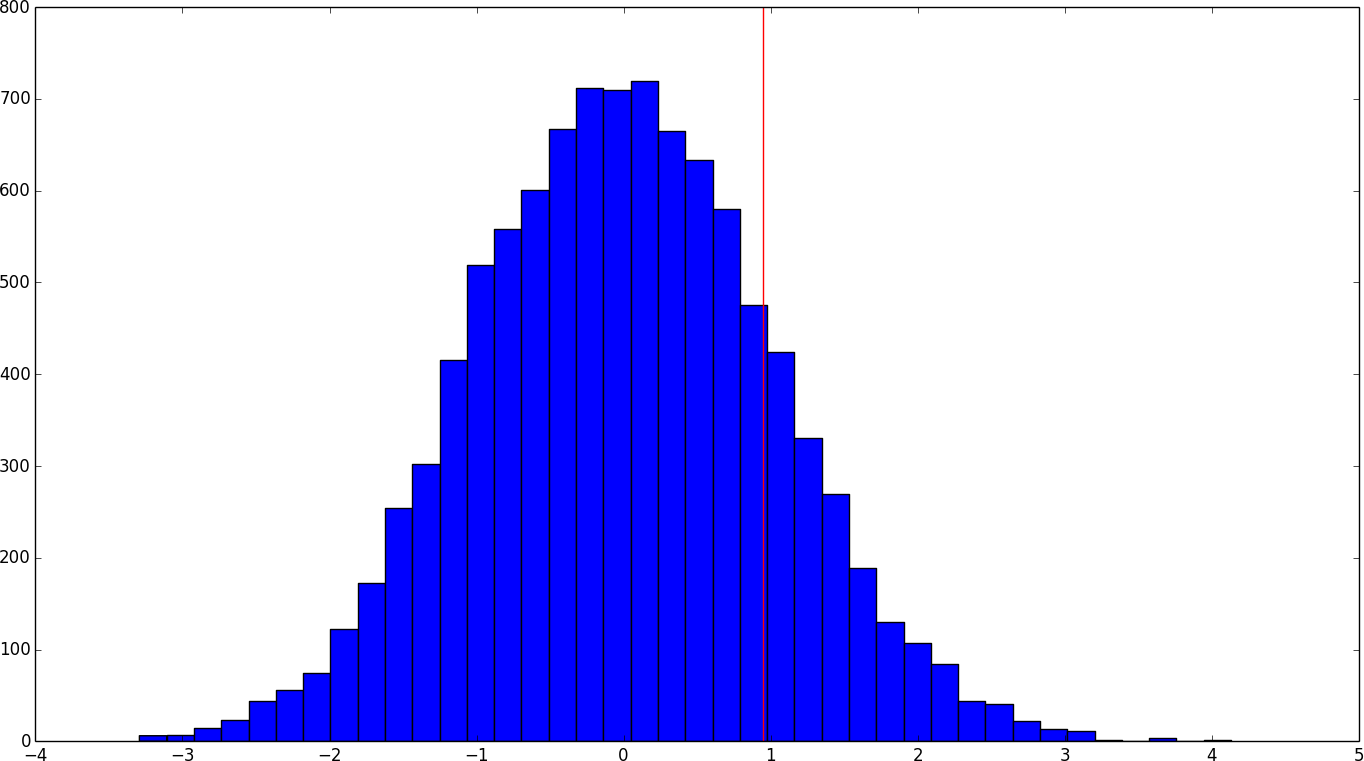
\includegraphics[width=.8\textwidth]{fig/figure_2.png}\par
  \end{centering}

  \caption{\label{fig:figure2}Permutation Null Distribution.}

\end{figure}



\end{document}
